\documentclass{article}

%Preamble
\title{CS 585 Assignment 2}
\author{Don Johnson}
\date{January 29, 2014}
\usepackage{graphicx}
\usepackage[margin=0.5in]{geometry}
\usepackage{listings}
\lstset{language=C}
\usepackage{caption}
\usepackage{subcaption}
\usepackage{underscore}
\usepackage{mathtools}

%Content
\begin{document}
\maketitle
\section{Assignment 2 (100 points)}
\subsection{Learning Objectives}
\subsection{Technical Task (30 points)}
Source code for technical task in ZIP file: Assignment2.cpp, Assignment2.hpp, Gui.cpp and Operators.cpp
\subsection{Programming Assignment Questions (28 points)}

\begin{enumerate}

\item
Run your program on the image yellowEgg.jpg both by thresholding the gradient magnitude and by using the Canny edge detector. Choose a threshold and smoothing level that leads to a nice contour and filled region of the egg. Saved edge and region-filled images below:

Note: Smoothing value units are one standard deviation and threshold values are pixel integer values. Unlike the gradient edge detector, the Canny has both a lower and upper threshold that I set to be threes times the lower threshold. Consequently, the Canny output files have two thresholds in their name.

\begin{figure}[ht!]
\centering
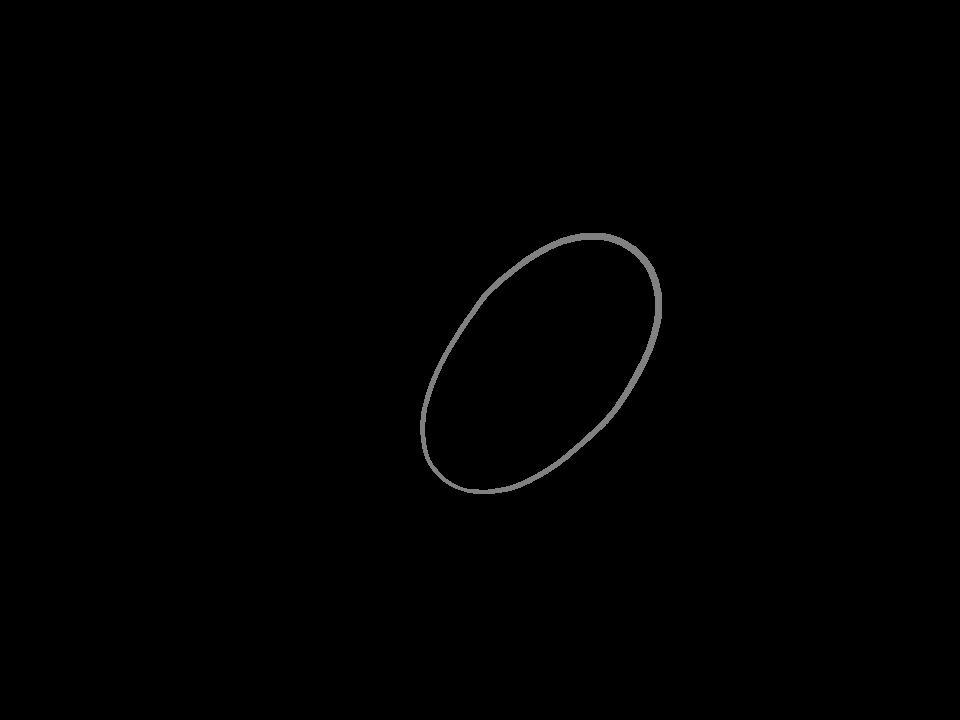
\includegraphics[width=100mm]{/Users/donj/workspace/cs585/Lab2/Mac/Assignment2/Data/SoloYellowEgg-Gradient-edges-2pt5-82.png}
\caption{SoloYellowEgg-Gradient-edges-2pt5-82.png}
\label{overflow}
\end{figure}

\begin{figure}[ht!]
\centering

\includegraphics[width=100mm]{/Users/donj/workspace/cs585/Lab2/Mac/Assignment2/Data/SoloYellowEgg-Gradient-result-2pt5-82.png}
\caption{SoloYellowEgg-Gradient-result-2pt5-82.png}
\label{overflow}
\end{figure}

\begin{figure}[ht!]
\centering
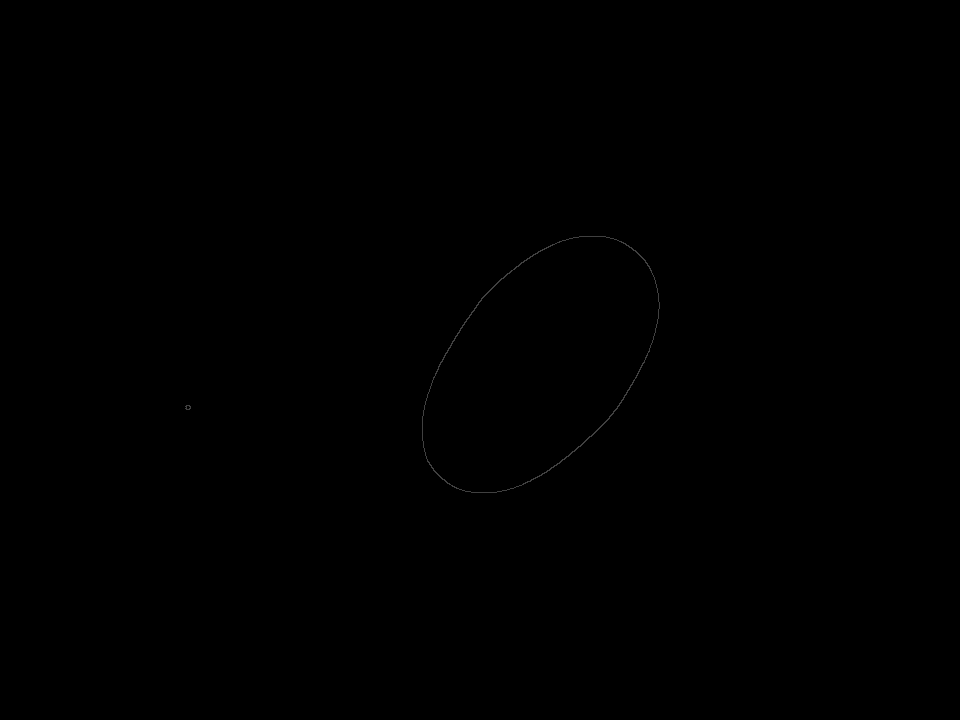
\includegraphics[width=100mm]{/Users/donj/workspace/cs585/Lab2/Mac/Assignment2/Data/SoloYellowEgg-Canny-edges-1-129-387.png}
\caption{SoloYellowEgg-Canny-edges-1-129-387.png}
\label{overflow}
\end{figure}

\begin{figure}[ht!]
\centering

\includegraphics[width=100mm]{/Users/donj/workspace/cs585/Lab2/Mac/Assignment2/Data/SoloYellowEgg-Canny-result-1-129-387.png}
\caption{SoloYellowEgg-Canny-result-1-129-387.png}
\label{overflow}
\end{figure}












\item
Since the red channel value for both a yellow and a red object are the same, the output of the thresholding program, which only looks at the red channel, will be the same.

\item
The results were what I expected based on the explanation in the previous item.
\begin{figure}[ht!]
\centering
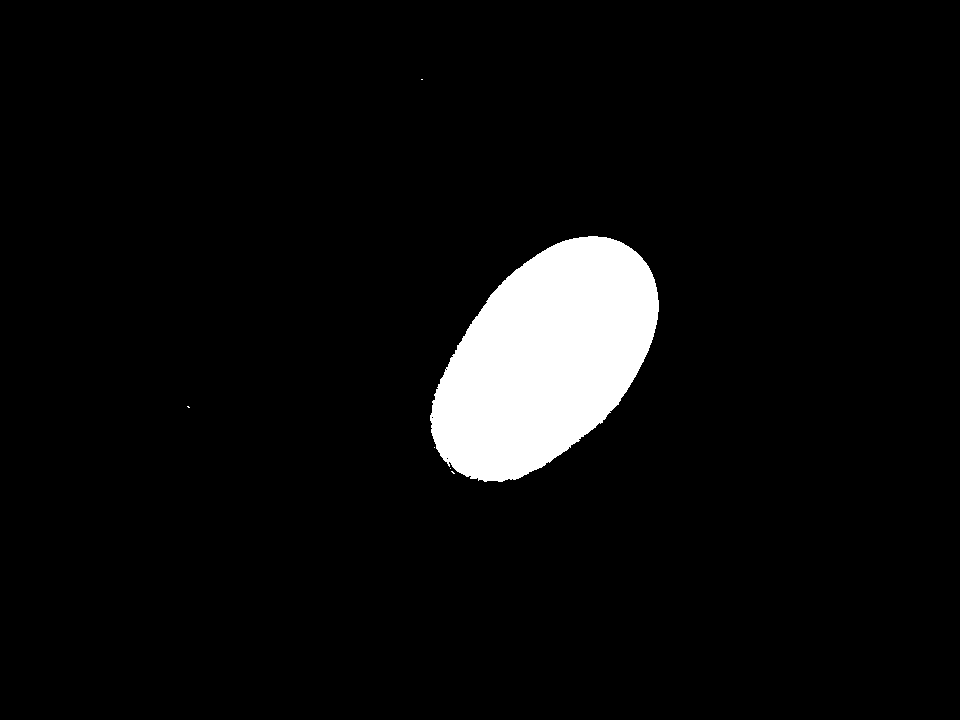
\includegraphics[width=100mm]{yellowEggThresholded175.png}
\caption{Mask Created by Red Threshold of Yellow Egg}
\label{overflow}
\end{figure}


\item
For a given pixel with RGB values, and ignoring the blue value, look at the ratio R/(R+G). Define "red" to be when the ration is greater than 2/3. Define "yellow" to be where the ratio is between 1/3 and 2/3. Exclude noise and shadow for red by requiring that the sum of red and green be greater than 100 and for yellow that the sum be greater than 300. Using these criteria and assigning 255 to red and 128 to yellow, I created this mask of the red and yellow egg image:
\begin{figure}[ht!]
\centering
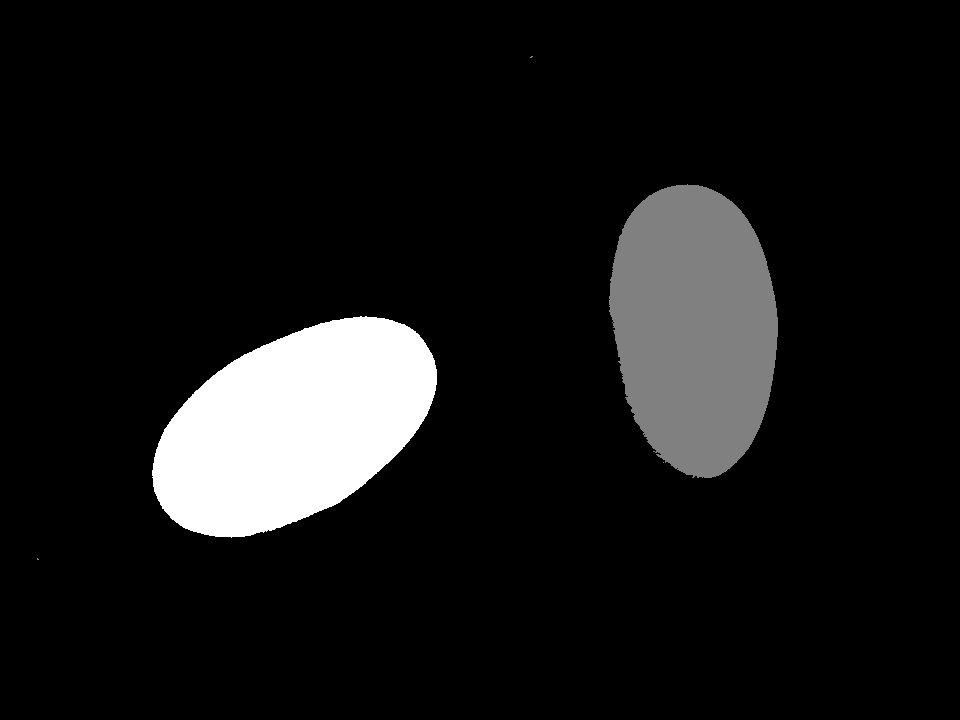
\includegraphics[width=100mm]{detectRedAndYellowEgg.png}
\caption{Detecting Red and Yellow Objects Using RGB Ratios (Red=White, Yellow=Gray)}
\label{overflow}
\end{figure}


This is a code snippet with the ratio logic:
\begin{lstlisting}
int indexGreen = col*channels + 1; // red
int indexRed = col*channels + 2; // green
int redPlusGreen = imagePtr[indexRed] + imagePtr[indexGreen]; 
float ratio = imagePtr[indexRed]/(redPlusGreen + 0.1);
channelPtr[col] = ratio > oneThird && redPlusGreen > 300 ? 128 : 0; 
channelPtr[col] = ratio > twoThirds && redPlusGreen > 100  ? 255 : channelPtr[col];
\end{lstlisting}

\item
Took a picture of my son's penguin, but against a white background to minimize difficulties. Also decided to try detecting yellow as well as red, but picked up white and gray so had to add two more lines to the previous code to eliminate pixels with blue RGB component greater than 100:
\begin{lstlisting}
int indexBlue = col*channels; // blue
channelPtr[col] = imagePtr[indexBlue] > 100  ? 0 : channelPtr[col];
\end{lstlisting}
The algorithm labeled the brighter part of the orange feet and my hand as yellow. Here are the original image and output mask:

\begin{figure}[h!]
\centering
\begin{subfigure}{.5\textwidth}
  \centering
  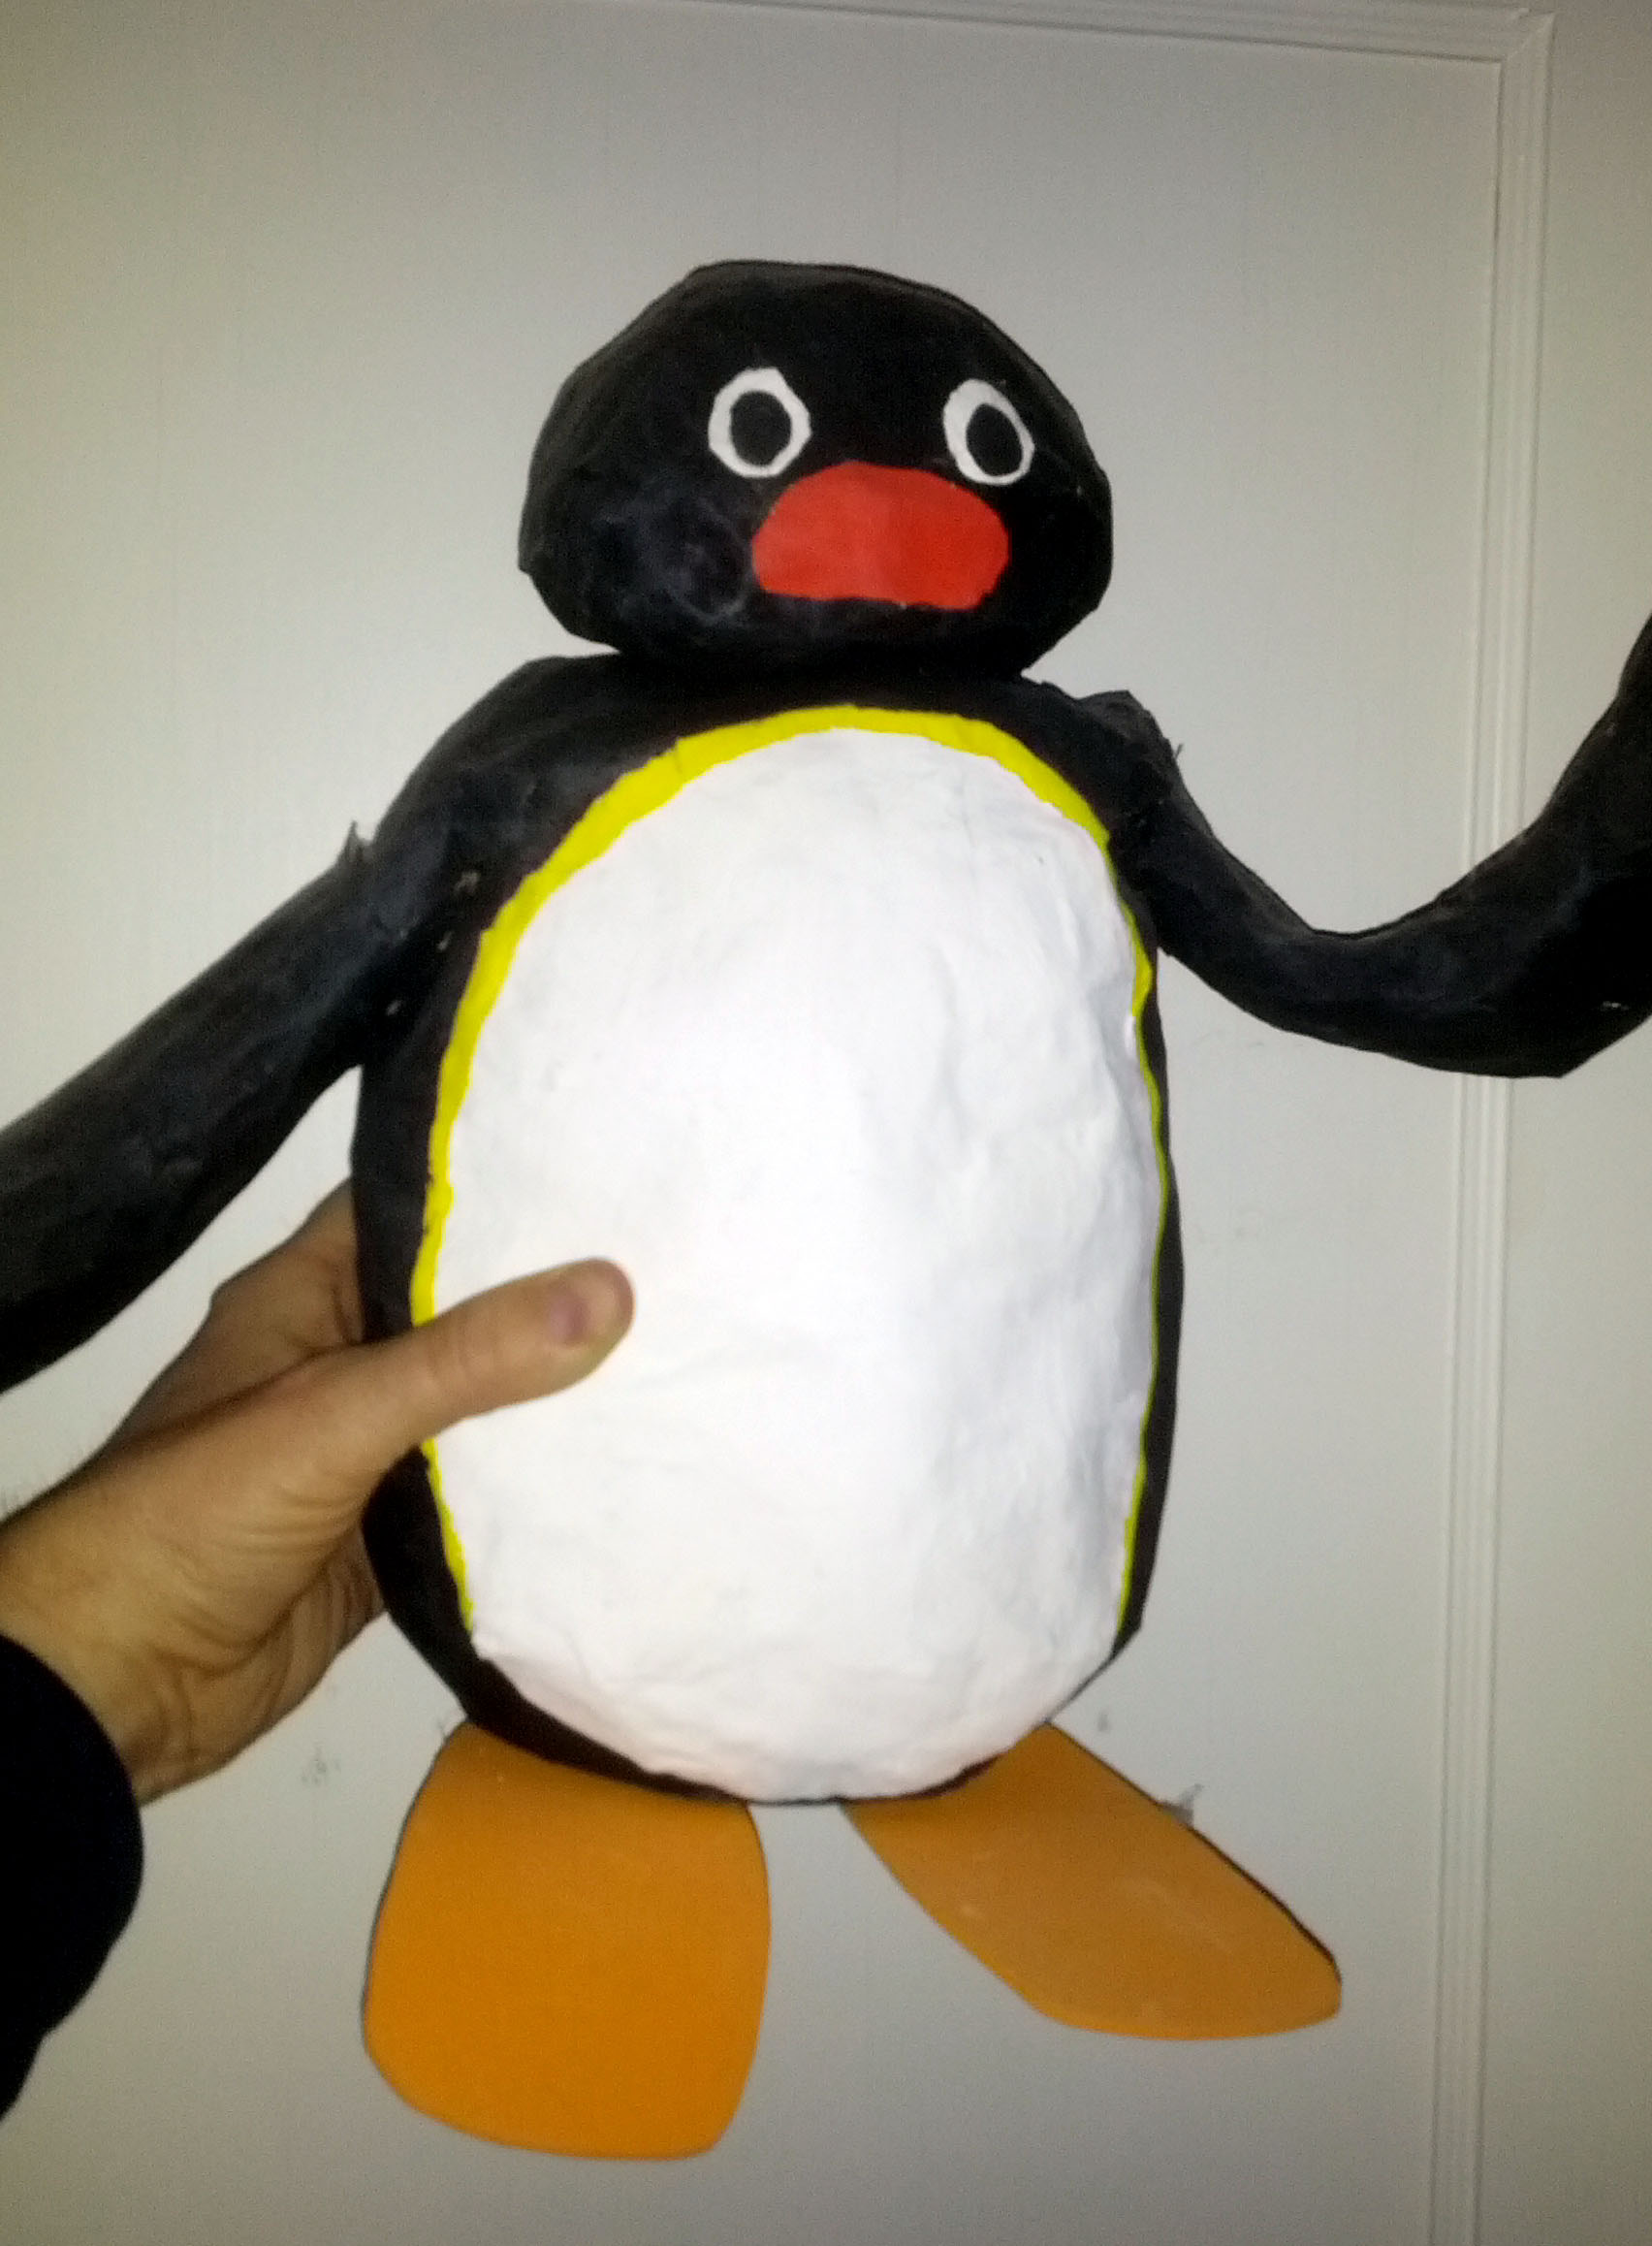
\includegraphics[width=80mm]{penguin.png}
  \caption{Original}
  \label{fig:sub1}
\end{subfigure}%
\begin{subfigure}{.5\textwidth}
  \centering
  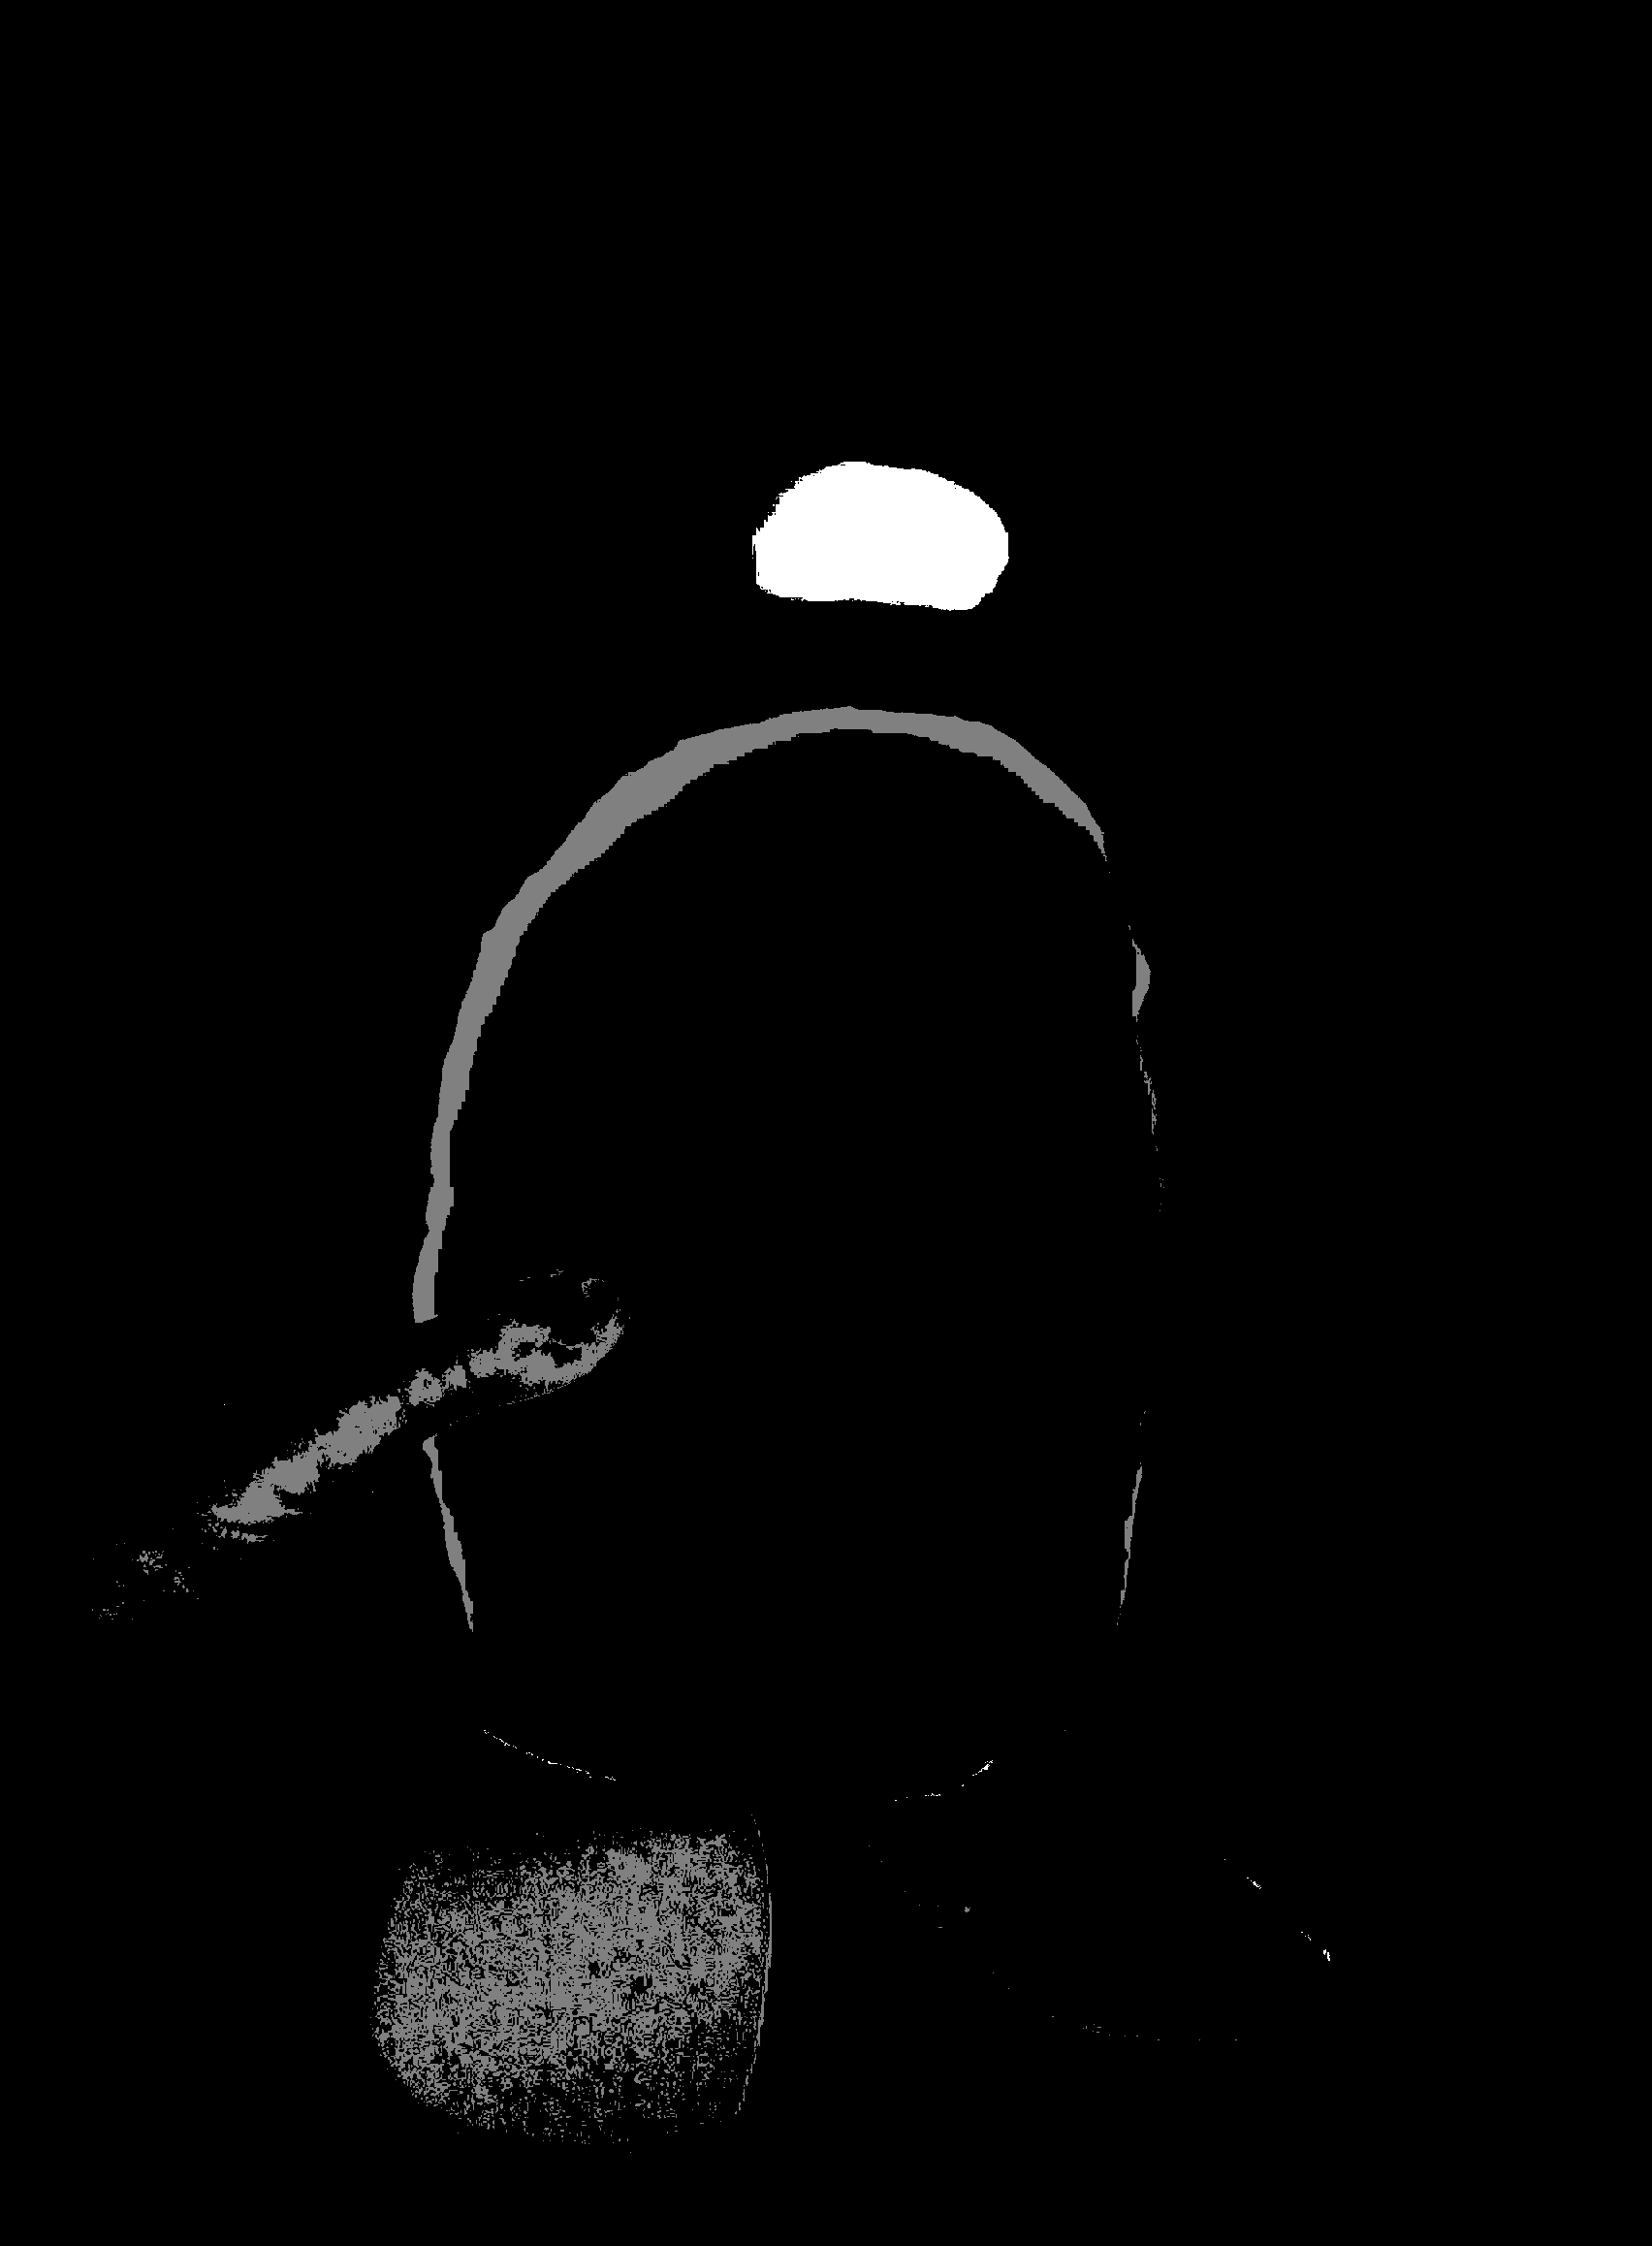
\includegraphics[width=80mm]{detectRedAndYellowOnPenguin.png}
  \caption{Mask with Red=White and Yellow=Gray}
  \label{fig:sub2}
\end{subfigure}
\caption{The Penguin}
\label{fig:test}
\end{figure}

\item
The color representation idea that I found most interesting was the trichromatic theory of perception where monochromatic colors, in terms of perception, can be created as a mixture of three primaries: 700 nm, 546 nm and 436 nm. Also, found the description of the CIE, XYZ color space and the matrix that relates it to the RGB space interesting.

\item
A monochromatic image of dimension 960x720 has 691,200 pixels. A RGB image of that size has 691,000 x 3 = 2073600 bytes, but still the same number of pixels.

\item
Found these timing values in the original code:

\begin{tabular}{| l | r |}
\hline
Name              & Elapsed Time (sec) \\
\hline
Linear Index v1  & 67.690270412808275   \\
\hline
Linear Index v2            & 21.070437060547910   \\
\hline
Linear Index v3           & 3.7960514995024437  \\
\hline
Row Ptr & 3.5284727421810489 \\
\hline
\end{tabular}

In the version 3, addOne_LinearIndex() function, the image.step[0] function is only being called 720 times, once per row. In the version 2, the image.step[0] function is being called 2,073,600 times, once per each channel in every pixel. Since image.step[0] always returns 2880, the number of bytes in a row, it can be moved outside of the loops in both versions of the addOne_LinearIndex() function. When you do this, the run times are almost identical:

\begin{tabular}{| l | r |}
\hline
Name              & Elapsed Time (sec) \\
\hline
Linear Index v2            & 3.9606397209834103   \\
\hline
Linear Index v3           & 3.8033933929887844  \\
\hline
\end{tabular}

Conclusion, run times differences between v2 and v3 of the addOne LinearIndex() function are caused by calls to the image.step[0] function and not by differing number of mathematical operations. As a side note, and not counting the pixel increment, v2 has two multiplications and two additions while v3 has only one multiplication and two additions per pixel. In the rainbowSpheres.jpg image we are using, there a 691,200 pixels so the various operation just mentioned happen one or two times that number. The slightly slower time of v2, once the step[] function has been removed may be caused by the extra multiplication it has over v3.

\item
This code snippet below demonstrates the strange thing that is happening in when we add 1 to a color channel of an image. If the color channel is saturated (equal to 255) for a particular pixel, the color channel value rolls over to 0 because it is a unsigned byte. This why the more saturated areas of the image showed a strange speckled effect. The color also changes. For example if you add one to a saturated green channel in a  yellow pixel, the pixel changes to red.
\newline\newline
Here is the code and output:
\begin{lstlisting}
unsigned char nvar = 253;
for(int i=0;i<5;i++){
    printf("nvar + 1: %d\n", (unsigned int)++nvar);
}
\end{lstlisting}

Output:
\newline
nvar + 1: 254
\newline
nvar + 1: 255
\newline
nvar + 1: 0   (Here is where the value rolled over)
\newline
nvar + 1: 1
\newline
nvar + 1: 2

\end{enumerate}

\section{Lecture preparation}
\subsection{Preparation for Lecture 2}
\begin{enumerate}
\item
Formula for the area A, of the base of a cone, given an apex angle \( \alpha \), and height h:
\begin{eqnarray*}
\tan \alpha =\frac{r}{h}
\\r=h \tan\alpha
\\A=\pi r^{2}
\\A=\pi\left ( h\tan\alpha \right )^{2}
\end{eqnarray*}

\item
Solving for side Z of the blue triangle using properties of similar triangles:
\begin{eqnarray*}
\frac{Z}{f}=\frac{X}{u}
\\Z=\frac{X}{u}\cdot f
\\Z=\frac{5000 mm \cdot 25 mm}{0.540 mm}
\\Z=231.48m
\end{eqnarray*}

\item
Solving for side u of the red triangle using properties of similar triangles:
\begin{eqnarray*}
\frac{Z}{f}=\frac{X}{u}
\\u=\frac{f}{X}\cdot Z
\\u=\frac{25 mm \cdot 1000 mm}{10000 mm}
\\u=2.5 mm
\end{eqnarray*}

\item
Count N in pixels of u in for an \(18 \mu m\) pixel is:
\begin{eqnarray*}
N=\frac{u}{pixels\:size\:in\:\mu m}
\\N=\frac{2500 \mu m}{18 \mu m}
\\N=139 pixels
\end{eqnarray*}

\item
The magnitude of the vectors, n, v:
\begin{eqnarray*}
\left | n \right |=\sqrt{\left( 1\right )^{2}+\left( 1\right )^{2}}=\sqrt{2}
\\\left | v \right |=\sqrt{\left( 1\right )^{2}+\left( 0.5\right )^{2}}=\frac{\sqrt{5}}{2}
\end{eqnarray*}
\newline
The corresponding unit vectors \(\left \| n \right \|, \left \| v \right \|\):
\begin{eqnarray*}
\left \| n \right \|=(\frac{1}{\sqrt{2}},\frac{1}{\sqrt{2}})
\\\left \| v \right \|=( \frac{2}{\sqrt{5}}, \frac{1}{\sqrt{5}} )
\end{eqnarray*}

\item
The dot product of unit vectors \(\left \| n \right \|, \left \| v \right \|\):
\begin{eqnarray*}
\left \| n \right \|\cdot \left \| v \right \|=\frac{1}{\sqrt{2}}\cdot\frac{2}{\sqrt{5}}+\frac{1}{\sqrt{2}}\cdot\frac{1}{\sqrt{5}}
\\\left \| n \right \|\cdot \left \| v \right \|=\frac{3}{\sqrt{10}}
\end{eqnarray*}

\item
The angle \(\theta\) between vectors n, v:
\begin{eqnarray*}
\cos \theta=\frac{n \cdot v}{\left | n \right | \cdot \left | v \right |}
\\\cos \theta=\frac{1\cdot1+1\cdot\frac{1}{2}}{\sqrt{2}\cdot\frac{\sqrt{5}}{2}}
\\\cos \theta=\frac{3}{\sqrt 10}
\\\theta=18.44^{\circ}
\end{eqnarray*}

\item
The projection p of v, onto n:
\begin{eqnarray*}
p=\left | v \right |\cos \theta\cdot\left \| n \right \|
\\p=\frac{\sqrt{5}}{2}\cdot\frac{3}{\sqrt 10}(\frac{1}{\sqrt{2}},\frac{1}{\sqrt{2}})
\\p=\frac{3}{2\sqrt 2}(\frac{1}{\sqrt{2}},\frac{1}{\sqrt{2}})
\\p=(\frac{3}{4},\frac{3}{4})
\end{eqnarray*}


\item
The perpendicular vector q, between v and n:
\begin{eqnarray*}
q=v-p
\\q=(1,\frac{1}{2})-(\frac{3}{4},\frac{3}{4})
\\q=(\frac{1}{4},-\frac{1}{4})
\end{eqnarray*}
Finally, r equals the sum of the components we just calculated:
\begin{eqnarray*}
r=p+q
\\r=(\frac{3}{4},\frac{3}{4})+(\frac{1}{4},-\frac{1}{4})
\\r=(\frac{1}{2},\frac{1}{2})
\end{eqnarray*}

\end{enumerate}

\subsection{Preparation for Lecture 3}
\begin{enumerate}
\item
Adapted from source: http://www.csl.mtu.edu/cs2321/www/newLectures/26_Depth_First_Search.html

\begin{lstlisting}
Definitions: 
G is a graph
G.incidentEdges(v) - all of the edges associated with vertex v
G.opposite(v,e) - a vertex at the other end of edge e connected to v

Note: Every edge and vertex is marked initially as unexplored.
The algorithm terminates when all vertices and edges have been explored.
The initial vertex is the root.

Algorithm for depth-first, recursive transversal of graph G:

DFS(graph G, Vertex v) 

for all edges e in G.incidentEdges(v) do

    if edge e is unexplored then
    
        w = G.opposite(v, e) 
        if vertex w is unexplored then 
            label e as discovery edge 
            recursively call DFS(G, w) 
        else 
            label e as a back edge
            
\end{lstlisting}

\item
Algorithm to find connected components of graph and using depth-first transversal algorithm in previous question:
\begin{lstlisting}
Given a set of vertices {a,b,c,d,e,...}

Create a 2-dimensional matrix where the row and columns are the labeled with the vertices.
A cell value of 1 means they are connected and 0 unconnected.
Initialize (a,a), (b,b),(c,c).... equal to 1 - every vertex is connected to itself.

for all vertices v in G
	Do DFS(G, v) only for sum of row and column with same label is greater than one
		
		for each v, treated as root vertex, set connection matrix cell (v,v1), (v,v2), (v,v3) equal to 1 when v1, v2, v3, ... are visited during algorithm. 	
\end{lstlisting}

\pagebreak
\item
\begin{figure}[ht!]
\centering
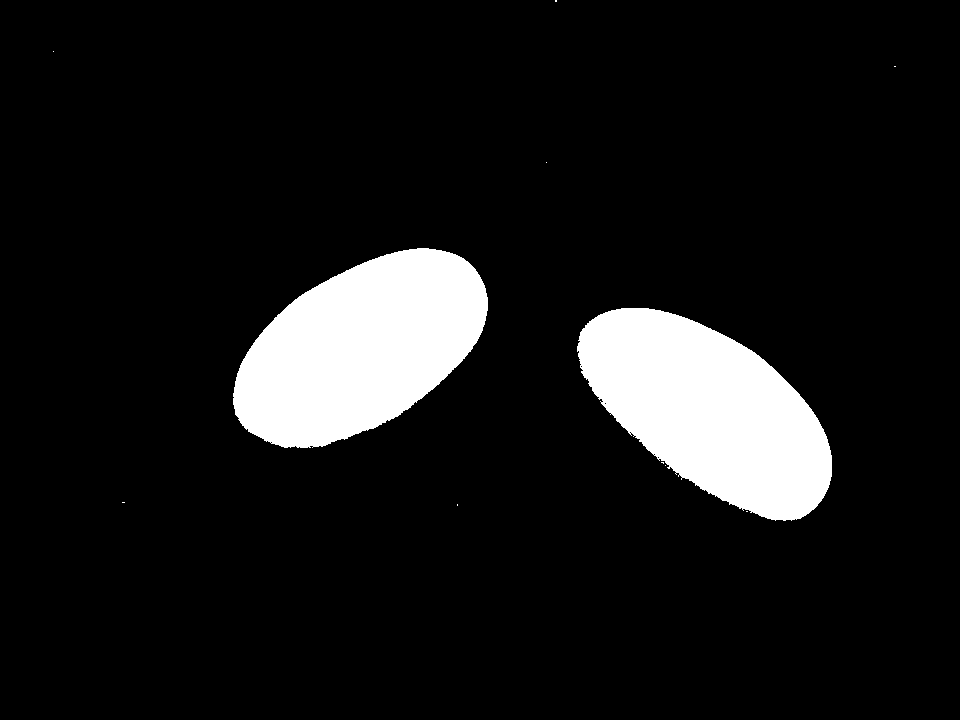
\includegraphics[width=100mm]{twoRedEggsThresholded175.png}
\caption{Results from running my program from section 1.2 on the picture "twoRedEggs.jpg"}
\label{overflow}
\end{figure}

\item
\begin{itemize}
\item
To find the number of red objects, I would define red for a pixel as a minimum ratio between the red channel and the blue, green channels
\item
Create a mask of all of those pixels defined as red, setting them equal to 1 and all other pixels equal to 0
\item
Run a depth first algorithm against the mask, visiting only the pixels equal to 1, treating each pixel as a vertex and each pixel boundary as an edge. Make it a greedy algorithm, collecting sets of connected pixels and keeping track of which pixels have been visited.
\item
Count the pixel sets to determine number of red objects
\end{itemize}
\item
My strategy for discarding the small extra regions that may pass through your red-object detector would be to require a minimal set size when counting the sets in the last step of the algorithm outlined in the previous question.

\item
If I was trying to create an rordered list of pixels that comprised the perimeter of an image region, for example, one of the red objects in the previous problem, I would:
\begin{itemize}
\item
Assume a x,y coordinate system for the image with (0,0) being the upper-left hand coordinate and both x and y increasing as you went down and to the right of the image.
\item
Find a pixel in one of the objects pixels sets from the previous problem with a value equal to 1 and having an x-coordinate minima in the set of pixels for that object. This will be one of the far left pixels in the object.
\item
Check for neighbor pixels with a value of one in this order: left, left-up, up, right-up, right, right-down, down, left-down
\item
When a non-zero neighbor is found, add it to a linked list, mark the pixel as visited and repeat the left to clockwise search pattern starting at the pixel boundary at which you entered.
\item
Repeat the process until you return to the first pixel where you started. The approach is similar to the approach used by bright physician from Egypt on the Maze of the Minotaur. The linked list contains the boundary pixels for the object.
\end{itemize}

\end{enumerate}

\end{document}
